\documentclass[12pt,letterpaper]{article}

\usepackage[utf8]{inputenc}
\usepackage[T1]{fontenc}
\usepackage{amsmath}
\usepackage{amsfonts}
\usepackage{amssymb}
\usepackage{amsthm}
\usepackage[left=2cm,right=2cm,top=2cm,bottom=2cm,headheight=22pt]{geometry}
\usepackage{fancyhdr}
\usepackage{setspace}
\usepackage{lastpage}
\usepackage{graphicx}
\usepackage{caption}
\usepackage{subcaption}
\usepackage{paralist}
\usepackage{url}
\usepackage{rotating}
\usepackage{pdfpages}

\theoremstyle{definition}
\newtheorem{question}{Question}
\newtheorem{example}{Example}
\newtheorem{exercise}[question]{Exercise}
\newtheorem*{challenge}{Challenge}
\newtheorem*{theorem}{Theorem}
\newtheorem*{definition}{Definition}

\begin{document}

%Paramètres de mise en forme des paragraphes selon les normes françaises
\setlength{\parskip}{1ex plus 0.5ex minus 0.2ex}
\setlength{\parindent}{0pt}

%Paramètres relatifs aux en-têtes et pieds de page.
\pagestyle{fancy}
\lhead{Theron J Hitchman}
\chead{\Large Reading and Guided Practice \#05}
\rhead{Spring 2016}
\lfoot{\emph{Math and Decision Making }}
\cfoot{}
\rfoot{\emph{\thepage\ of \pageref{LastPage}}}

\section*{Introduction}

Here you will learn about several other puzzles that can be turned into a graph theory question. 
You will practice the process of ``abstracting away'' inessential details while keeping the important parts, 
and you will run across another invention of Leonhard Euler.

\section*{Goals}
At the end of this assignment, a student should be able to:
\begin{compactitem}
\item Describe what a \emph{multigraph} is, and how that differs from a graph.
\item Describe what an \emph{Eulerian Cycle} is.
\item Describe what an \emph{Eulerian Graph} is.
\end{compactitem}
A student might also be able to:
\begin{compactitem}
\item Solve several challenging puzzles involving Eulerian Cycles.
\end{compactitem}

\section*{Reading and Questions for Graphs Day 6}

\subsection*{Another Puzzle, Euler, and the process of Abstraction}

The people of the city of K\"{o}nigsberg (which since 1945 is called Kaliningrad), liked to walk in the evenings. It
was a social event. The city is built on the banks of a river (now called the \emph{Pregolya}), and includes some
islands in the middle of that river. What is interesting is that the city had seven bridges joining the various
land masses, and you could stroll across them to enjoy the view of the river during your walk. So people began
to wonder:
\begin{quote}
Is it possible to take a walk around the city in a way that crosses each bridge exactly once, and return to the
place you started?
\end{quote}

On the next page is Figure \ref{figure:konigsberg}, a map of Kaliningrad I got from Google Maps. But things have changed since the puzzle was solved, and only five of the original seven bridges are still standing. So, I have marked those five bridges, and also added marks for spots which are approximately where the other two bridges used to be.

\begin{challenge}Can you solve the K\"{o}nigsberg Bridges Puzzle?
\end{challenge}

\clearpage

\begin{figure}[h]
\centering
\begin{sideways}
\includegraphics[width=.4\textwidth]{images/konigsberg.pdf}
\end{sideways}
\caption{Kaliningrad, with the bridges of K\"{o}nigsberg}
\label{figure:konigsberg}
\end{figure}

In 1736, Leonhard Euler was Professor of Mathematics at the Imperial Russian Academy of Sciences, and served as
kind of a court mathematician for the Russian Csar. As a bit of a diversion, he took up the K\"{o}nigsberg Bridges
problem.  His method of solution involved changing the puzzle into one about the properties of a graph, and then
figuring that out instead.

Euler realized that most of the map is completely unnecessary. The essential features of the puzzle are these:
\begin{compactitem}
\item some land masses,
\item some bridges joining them, and
\item the problem is make a path to start and end at the same bit of land while crossing all of the bridges.
\end{compactitem}

So, he threw everything else out. For the land, he drew some dots, which we call vertices. For the bridges, he
drew connections between the vertices, which we call edges. You get this kind of picture:

\begin{figure}[h]
\centering
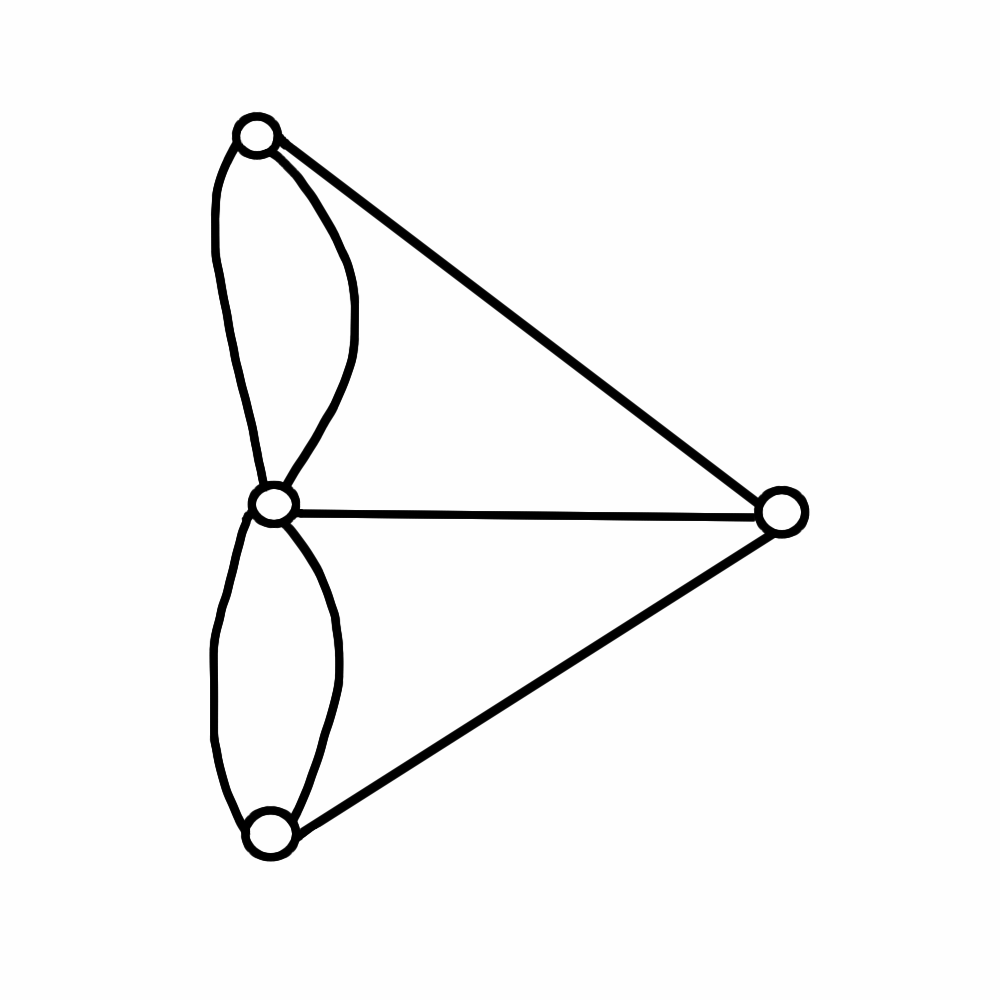
\includegraphics[width=.3\textwidth]{images/konigsberg-graph.png}
\caption{Euler's K\"{o}nigsberg Graph}
\label{figure:konigsberg-graph}
\end{figure}

\begin{exercise}
Take a good look and see how the land masses and the bridges work out to the same set of connective 
relationships.
\end{exercise}

With this change, what does the puzzle say now? It should read something like this.
\begin{quote}
Is there a cycle on the graph in Figure \ref{figure:konigsberg-graph} which uses each edge exactly once?
\end{quote}

These days, such a thing is named after Euler, to honor him. An \emph{Eulerian cycle} is a cycle which uses every
edge of the graph exactly once. A graph is called an \emph{Eulerian graph} if it has an Eulerian cycle.

What Euler proceeded to do was prove that the graph in Figure \ref{figure:konigsberg-graph} does not have
an Eulerian cycle. So, the people of K\"{o}nigsberg were stuck. The puzzle is impossible.

\begin{challenge}
What feature of the graph in Figure \ref{figure:konigsberg-graph} makes it impossible to have an
Eulerian cycle?
\end{challenge}

\begin{exercise}
Draw two different graphs which definitely \textbf{do} have Eulerian cycles.
Be sure to write down how to walk on the cycle so you don't forget.
\end{exercise}


\subsection*{A Subtle Generalization}

Did you notice something a little bit ``off?'' Take a good hard look at the graph in Figure \ref{figure:konigsberg-graph}. 

There are pairs of vertices which have more than one edge joining them! We haven't really drawn these kinds of 
examples before. Though I guess they weren't explicitly disallowed by our definition. Some people don't allow these
kind of multiple edge situations. In that case, Figure \ref{figure:konigsberg-graph} is not technically a graph any more, and instead, people will call it a \emph{multi-graph}.

\subsection*{Two more puzzles}

The last two pages of this reading each have a puzzle on them. Those puzzles are related, to each other and to the 
K\"{o}nigsberg Bridges Puzzle. For each of them, do the next exercise.

\begin{exercise}
Go through the process of abstracting away the inessential details of the puzzle.
Find the essential features of the problem. What are the ``things'' you are connecting, and what are the ``connections'' between them. Use this to turn the problem into one about graph theory.
Draw the graph that matters. Restate the puzzle as a puzzle about your graph.
\end{exercise}

\begin{challenge}
Find a solution to the puzzle, if you can. Find a way to describe why it is impossible, if you cannot.
\end{challenge}

\clearpage

\includepdf[pages=2-3]{mdm-graphs-handout-day05.pdf}



%\begin{thebibliography}{9}
%\end{thebibliography}

\end{document}
%sagemathcloud={"zoom_width":100}